\documentclass[twoside]{book}

% Packages required by doxygen
\usepackage{fixltx2e}
\usepackage{calc}
\usepackage{doxygen}
\usepackage[export]{adjustbox} % also loads graphicx
\usepackage{graphicx}
\usepackage[utf8]{inputenc}
\usepackage{makeidx}
\usepackage{multicol}
\usepackage{multirow}
\PassOptionsToPackage{warn}{textcomp}
\usepackage{textcomp}
\usepackage[nointegrals]{wasysym}
\usepackage[table]{xcolor}

% Font selection
\usepackage[T1]{fontenc}
\usepackage[scaled=.90]{helvet}
\usepackage{courier}
\usepackage{amssymb}
\usepackage{sectsty}
\renewcommand{\familydefault}{\sfdefault}
\allsectionsfont{%
  \fontseries{bc}\selectfont%
  \color{darkgray}%
}
\renewcommand{\DoxyLabelFont}{%
  \fontseries{bc}\selectfont%
  \color{darkgray}%
}
\newcommand{\+}{\discretionary{\mbox{\scriptsize$\hookleftarrow$}}{}{}}

% Page & text layout
\usepackage{geometry}
\geometry{%
  a4paper,%
  top=2.5cm,%
  bottom=2.5cm,%
  left=2.5cm,%
  right=2.5cm%
}
\tolerance=750
\hfuzz=15pt
\hbadness=750
\setlength{\emergencystretch}{15pt}
\setlength{\parindent}{0cm}
\setlength{\parskip}{3ex plus 2ex minus 2ex}
\makeatletter
\renewcommand{\paragraph}{%
  \@startsection{paragraph}{4}{0ex}{-1.0ex}{1.0ex}{%
    \normalfont\normalsize\bfseries\SS@parafont%
  }%
}
\renewcommand{\subparagraph}{%
  \@startsection{subparagraph}{5}{0ex}{-1.0ex}{1.0ex}{%
    \normalfont\normalsize\bfseries\SS@subparafont%
  }%
}
\makeatother

% Headers & footers
\usepackage{fancyhdr}
\pagestyle{fancyplain}
\fancyhead[LE]{\fancyplain{}{\bfseries\thepage}}
\fancyhead[CE]{\fancyplain{}{}}
\fancyhead[RE]{\fancyplain{}{\bfseries\leftmark}}
\fancyhead[LO]{\fancyplain{}{\bfseries\rightmark}}
\fancyhead[CO]{\fancyplain{}{}}
\fancyhead[RO]{\fancyplain{}{\bfseries\thepage}}
\fancyfoot[LE]{\fancyplain{}{}}
\fancyfoot[CE]{\fancyplain{}{}}
\fancyfoot[RE]{\fancyplain{}{\bfseries\scriptsize Generated by Doxygen }}
\fancyfoot[LO]{\fancyplain{}{\bfseries\scriptsize Generated by Doxygen }}
\fancyfoot[CO]{\fancyplain{}{}}
\fancyfoot[RO]{\fancyplain{}{}}
\renewcommand{\footrulewidth}{0.4pt}
\renewcommand{\chaptermark}[1]{%
  \markboth{#1}{}%
}
\renewcommand{\sectionmark}[1]{%
  \markright{\thesection\ #1}%
}

% Indices & bibliography
\usepackage{natbib}
\usepackage[titles]{tocloft}
\setcounter{tocdepth}{3}
\setcounter{secnumdepth}{5}
\makeindex

% Hyperlinks (required, but should be loaded last)
\usepackage{ifpdf}
\ifpdf
  \usepackage[pdftex,pagebackref=true]{hyperref}
\else
  \usepackage[ps2pdf,pagebackref=true]{hyperref}
\fi
\hypersetup{%
  colorlinks=true,%
  linkcolor=blue,%
  citecolor=blue,%
  unicode%
}

% Custom commands
\newcommand{\clearemptydoublepage}{%
  \newpage{\pagestyle{empty}\cleardoublepage}%
}

\usepackage{caption}
\captionsetup{labelsep=space,justification=centering,font={bf},singlelinecheck=off,skip=4pt,position=top}

%===== C O N T E N T S =====

\begin{document}

% Titlepage & ToC
\hypersetup{pageanchor=false,
             bookmarksnumbered=true,
             pdfencoding=unicode
            }
\pagenumbering{roman}
\begin{titlepage}
\vspace*{7cm}
\begin{center}%
{\Large My Project }\\
\vspace*{1cm}
{\large Generated by Doxygen 1.8.11}\\
\end{center}
\end{titlepage}
\clearemptydoublepage
\tableofcontents
\clearemptydoublepage
\pagenumbering{arabic}
\hypersetup{pageanchor=true}

%--- Begin generated contents ---
\chapter{Namespace Index}
\section{Packages}
Here are the packages with brief descriptions (if available)\+:\begin{DoxyCompactList}
\item\contentsline{section}{\hyperlink{namespace_plex_byte}{Plex\+Byte} }{\pageref{namespace_plex_byte}}{}
\item\contentsline{section}{\hyperlink{namespace_plex_byte_1_1_mo_cap}{Plex\+Byte.\+Mo\+Cap} }{\pageref{namespace_plex_byte_1_1_mo_cap}}{}
\item\contentsline{section}{\hyperlink{namespace_plex_byte_1_1_mo_cap_1_1_backend}{Plex\+Byte.\+Mo\+Cap.\+Backend} }{\pageref{namespace_plex_byte_1_1_mo_cap_1_1_backend}}{}
\end{DoxyCompactList}

\chapter{Hierarchical Index}
\section{Class Hierarchy}
This inheritance list is sorted roughly, but not completely, alphabetically\+:\begin{DoxyCompactList}
\item I\+Disposable\begin{DoxyCompactList}
\item \contentsline{section}{Plex\+Byte.\+Mo\+Cap.\+Backend.\+Backend\+Service}{\pageref{class_plex_byte_1_1_mo_cap_1_1_backend_1_1_backend_service}}{}
\end{DoxyCompactList}
\end{DoxyCompactList}

\chapter{Class Index}
\section{Class List}
Here are the classes, structs, unions and interfaces with brief descriptions\+:\begin{DoxyCompactList}
\item\contentsline{section}{\hyperlink{class_plex_byte_1_1_mo_cap_1_1_interactions_1_1_account}{Plex\+Byte.\+Mo\+Cap.\+Interactions.\+Account} }{\pageref{class_plex_byte_1_1_mo_cap_1_1_interactions_1_1_account}}{}
\item\contentsline{section}{\hyperlink{class_plex_byte_1_1_mo_cap_1_1_interactions_1_1_expense}{Plex\+Byte.\+Mo\+Cap.\+Interactions.\+Expense} }{\pageref{class_plex_byte_1_1_mo_cap_1_1_interactions_1_1_expense}}{}
\item\contentsline{section}{\hyperlink{interface_plex_byte_1_1_mo_cap_1_1_interactions_1_1_i_account}{Plex\+Byte.\+Mo\+Cap.\+Interactions.\+I\+Account} }{\pageref{interface_plex_byte_1_1_mo_cap_1_1_interactions_1_1_i_account}}{}
\item\contentsline{section}{\hyperlink{interface_plex_byte_1_1_mo_cap_1_1_interactions_1_1_i_expense}{Plex\+Byte.\+Mo\+Cap.\+Interactions.\+I\+Expense} }{\pageref{interface_plex_byte_1_1_mo_cap_1_1_interactions_1_1_i_expense}}{}
\item\contentsline{section}{\hyperlink{interface_plex_byte_1_1_mo_cap_1_1_interactions_1_1_i_interaction}{Plex\+Byte.\+Mo\+Cap.\+Interactions.\+I\+Interaction} }{\pageref{interface_plex_byte_1_1_mo_cap_1_1_interactions_1_1_i_interaction}}{}
\item\contentsline{section}{\hyperlink{interface_plex_byte_1_1_mo_cap_1_1_interactions_1_1_i_interaction_factory}{Plex\+Byte.\+Mo\+Cap.\+Interactions.\+I\+Interaction\+Factory} }{\pageref{interface_plex_byte_1_1_mo_cap_1_1_interactions_1_1_i_interaction_factory}}{}
\item\contentsline{section}{\hyperlink{class_plex_byte_1_1_mo_cap_1_1_interactions_1_1_interaction}{Plex\+Byte.\+Mo\+Cap.\+Interactions.\+Interaction} }{\pageref{class_plex_byte_1_1_mo_cap_1_1_interactions_1_1_interaction}}{}
\item\contentsline{section}{\hyperlink{class_plex_byte_1_1_mo_cap_1_1_interactions_1_1_interaction_event_args}{Plex\+Byte.\+Mo\+Cap.\+Interactions.\+Interaction\+Event\+Args} }{\pageref{class_plex_byte_1_1_mo_cap_1_1_interactions_1_1_interaction_event_args}}{}
\item\contentsline{section}{\hyperlink{class_plex_byte_1_1_mo_cap_1_1_interactions_1_1_interaction_factory}{Plex\+Byte.\+Mo\+Cap.\+Interactions.\+Interaction\+Factory} }{\pageref{class_plex_byte_1_1_mo_cap_1_1_interactions_1_1_interaction_factory}}{}
\item\contentsline{section}{\hyperlink{interface_plex_byte_1_1_mo_cap_1_1_interactions_1_1_i_object_factory}{Plex\+Byte.\+Mo\+Cap.\+Interactions.\+I\+Object\+Factory} }{\pageref{interface_plex_byte_1_1_mo_cap_1_1_interactions_1_1_i_object_factory}}{}
\item\contentsline{section}{\hyperlink{interface_plex_byte_1_1_mo_cap_1_1_interactions_1_1_i_project}{Plex\+Byte.\+Mo\+Cap.\+Interactions.\+I\+Project} }{\pageref{interface_plex_byte_1_1_mo_cap_1_1_interactions_1_1_i_project}}{}
\item\contentsline{section}{\hyperlink{interface_plex_byte_1_1_mo_cap_1_1_interactions_1_1_i_survey}{Plex\+Byte.\+Mo\+Cap.\+Interactions.\+I\+Survey} }{\pageref{interface_plex_byte_1_1_mo_cap_1_1_interactions_1_1_i_survey}}{}
\item\contentsline{section}{\hyperlink{interface_plex_byte_1_1_mo_cap_1_1_interactions_1_1_i_survey_option}{Plex\+Byte.\+Mo\+Cap.\+Interactions.\+I\+Survey\+Option} \\*The survey option interface }{\pageref{interface_plex_byte_1_1_mo_cap_1_1_interactions_1_1_i_survey_option}}{}
\item\contentsline{section}{\hyperlink{interface_plex_byte_1_1_mo_cap_1_1_interactions_1_1_i_task}{Plex\+Byte.\+Mo\+Cap.\+Interactions.\+I\+Task} }{\pageref{interface_plex_byte_1_1_mo_cap_1_1_interactions_1_1_i_task}}{}
\item\contentsline{section}{\hyperlink{interface_plex_byte_1_1_mo_cap_1_1_interactions_1_1_i_timeslice}{Plex\+Byte.\+Mo\+Cap.\+Interactions.\+I\+Timeslice} }{\pageref{interface_plex_byte_1_1_mo_cap_1_1_interactions_1_1_i_timeslice}}{}
\item\contentsline{section}{\hyperlink{interface_plex_byte_1_1_mo_cap_1_1_interactions_1_1_i_vote}{Plex\+Byte.\+Mo\+Cap.\+Interactions.\+I\+Vote} \\*The vote interface }{\pageref{interface_plex_byte_1_1_mo_cap_1_1_interactions_1_1_i_vote}}{}
\item\contentsline{section}{\hyperlink{class_plex_byte_1_1_mo_cap_1_1_interactions_1_1_object_factory}{Plex\+Byte.\+Mo\+Cap.\+Interactions.\+Object\+Factory} }{\pageref{class_plex_byte_1_1_mo_cap_1_1_interactions_1_1_object_factory}}{}
\item\contentsline{section}{\hyperlink{class_plex_byte_1_1_mo_cap_1_1_interactions_1_1_project}{Plex\+Byte.\+Mo\+Cap.\+Interactions.\+Project} }{\pageref{class_plex_byte_1_1_mo_cap_1_1_interactions_1_1_project}}{}
\item\contentsline{section}{\hyperlink{class_plex_byte_1_1_mo_cap_1_1_interactions_1_1_survey}{Plex\+Byte.\+Mo\+Cap.\+Interactions.\+Survey} }{\pageref{class_plex_byte_1_1_mo_cap_1_1_interactions_1_1_survey}}{}
\item\contentsline{section}{\hyperlink{class_plex_byte_1_1_mo_cap_1_1_interactions_1_1_survey_option}{Plex\+Byte.\+Mo\+Cap.\+Interactions.\+Survey\+Option} \\*The survey option class, which hold the option text }{\pageref{class_plex_byte_1_1_mo_cap_1_1_interactions_1_1_survey_option}}{}
\item\contentsline{section}{\hyperlink{class_plex_byte_1_1_mo_cap_1_1_interactions_1_1_task}{Plex\+Byte.\+Mo\+Cap.\+Interactions.\+Task} }{\pageref{class_plex_byte_1_1_mo_cap_1_1_interactions_1_1_task}}{}
\item\contentsline{section}{\hyperlink{class_plex_byte_1_1_mo_cap_1_1_interactions_1_1_timeslice}{Plex\+Byte.\+Mo\+Cap.\+Interactions.\+Timeslice} }{\pageref{class_plex_byte_1_1_mo_cap_1_1_interactions_1_1_timeslice}}{}
\item\contentsline{section}{\hyperlink{class_plex_byte_1_1_mo_cap_1_1_interactions_1_1_vote}{Plex\+Byte.\+Mo\+Cap.\+Interactions.\+Vote} \\*This class holds information about a users choice, containing the user and his choice selected }{\pageref{class_plex_byte_1_1_mo_cap_1_1_interactions_1_1_vote}}{}
\end{DoxyCompactList}

\chapter{File Index}
\section{File List}
Here is a list of all files with brief descriptions\+:\begin{DoxyCompactList}
\item\contentsline{section}{D\+:/\+Users/\+Christian\+B/\+Documents/\+\_\+\+H\+F Infomatik/\+Git\+Hub\+\_\+\+Repos/\+Mo\+Cap/\+Plex\+Byte.\+Mo\+Cap/\+Plex\+Byte.\+Mo\+Cap.\+Backend/\hyperlink{_backend_service_8cs}{Backend\+Service.\+cs} }{\pageref{_backend_service_8cs}}{}
\end{DoxyCompactList}

\chapter{Namespace Documentation}
\hypertarget{namespace_plex_byte}{}\section{Plex\+Byte Namespace Reference}
\label{namespace_plex_byte}\index{Plex\+Byte@{Plex\+Byte}}
\subsection*{Namespaces}
\begin{DoxyCompactItemize}
\item 
namespace \hyperlink{namespace_plex_byte_1_1_mo_cap}{Mo\+Cap}
\end{DoxyCompactItemize}

\hypertarget{namespace_plex_byte_1_1_mo_cap}{}\section{Plex\+Byte.\+Mo\+Cap Namespace Reference}
\label{namespace_plex_byte_1_1_mo_cap}\index{Plex\+Byte.\+Mo\+Cap@{Plex\+Byte.\+Mo\+Cap}}
\subsection*{Namespaces}
\begin{DoxyCompactItemize}
\item 
namespace \hyperlink{namespace_plex_byte_1_1_mo_cap_1_1_win_forms}{Win\+Forms}
\end{DoxyCompactItemize}

\hypertarget{namespace_plex_byte_1_1_mo_cap_1_1_security}{}\section{Plex\+Byte.\+Mo\+Cap.\+Security Namespace Reference}
\label{namespace_plex_byte_1_1_mo_cap_1_1_security}\index{Plex\+Byte.\+Mo\+Cap.\+Security@{Plex\+Byte.\+Mo\+Cap.\+Security}}
\subsection*{Classes}
\begin{DoxyCompactItemize}
\item 
interface \hyperlink{interface_plex_byte_1_1_mo_cap_1_1_security_1_1_i_person}{I\+Person}
\item 
interface \hyperlink{interface_plex_byte_1_1_mo_cap_1_1_security_1_1_i_user}{I\+User}
\item 
class \hyperlink{class_plex_byte_1_1_mo_cap_1_1_security_1_1_user}{User}
\end{DoxyCompactItemize}

\chapter{Class Documentation}
\hypertarget{interface_plex_byte_1_1_mo_cap_1_1_security_1_1_i_person}{}\section{Plex\+Byte.\+Mo\+Cap.\+Security.\+I\+Person Interface Reference}
\label{interface_plex_byte_1_1_mo_cap_1_1_security_1_1_i_person}\index{Plex\+Byte.\+Mo\+Cap.\+Security.\+I\+Person@{Plex\+Byte.\+Mo\+Cap.\+Security.\+I\+Person}}
Inheritance diagram for Plex\+Byte.\+Mo\+Cap.\+Security.\+I\+Person\+:\begin{figure}[H]
\begin{center}
\leavevmode
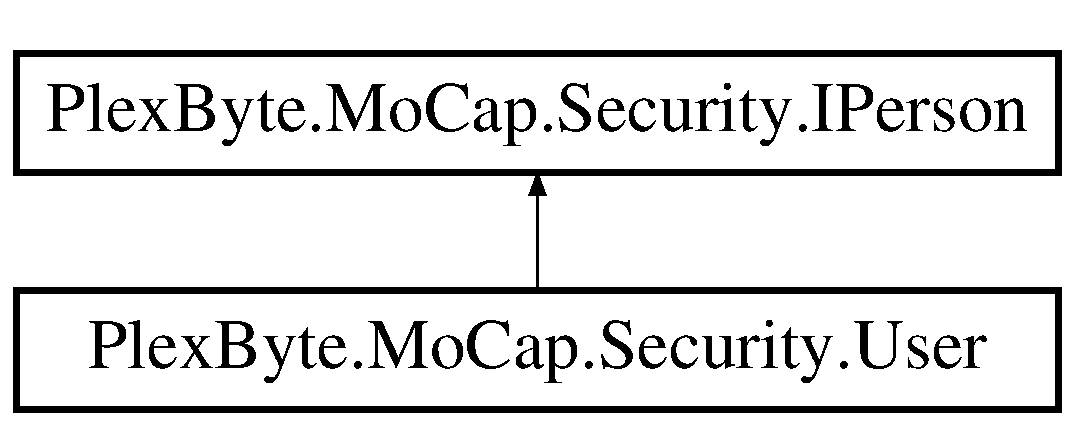
\includegraphics[height=2.000000cm]{interface_plex_byte_1_1_mo_cap_1_1_security_1_1_i_person}
\end{center}
\end{figure}
\subsection*{Properties}
\begin{DoxyCompactItemize}
\item 
string \hyperlink{interface_plex_byte_1_1_mo_cap_1_1_security_1_1_i_person_ac9e7eb738b289315473d898eef447acf}{Id}\hspace{0.3cm}{\ttfamily  \mbox{[}get\mbox{]}}
\item 
string \hyperlink{interface_plex_byte_1_1_mo_cap_1_1_security_1_1_i_person_aeddc80d36377ce378de21a5aea8ac574}{First\+Name}\hspace{0.3cm}{\ttfamily  \mbox{[}get, set\mbox{]}}
\item 
string \hyperlink{interface_plex_byte_1_1_mo_cap_1_1_security_1_1_i_person_ab4e080812cf1517ef2e3a56295b0965d}{Last\+Name}\hspace{0.3cm}{\ttfamily  \mbox{[}get, set\mbox{]}}
\item 
string \hyperlink{interface_plex_byte_1_1_mo_cap_1_1_security_1_1_i_person_aa42342d7ddfa8f866c9b64d655e04f26}{Middle\+Name}\hspace{0.3cm}{\ttfamily  \mbox{[}get, set\mbox{]}}
\item 
string \hyperlink{interface_plex_byte_1_1_mo_cap_1_1_security_1_1_i_person_a4662f6c71cabe18c5448e8d0c34a3c62}{Email\+Address}\hspace{0.3cm}{\ttfamily  \mbox{[}get, set\mbox{]}}
\item 
Date\+Time \hyperlink{interface_plex_byte_1_1_mo_cap_1_1_security_1_1_i_person_a4cb33b61b1369fadd6c47c15754e8b46}{Birthdate}\hspace{0.3cm}{\ttfamily  \mbox{[}get, set\mbox{]}}
\item 
Date\+Time \hyperlink{interface_plex_byte_1_1_mo_cap_1_1_security_1_1_i_person_a56f8b21246addbb7558331981695724f}{Created\+Date\+Time}\hspace{0.3cm}{\ttfamily  \mbox{[}get\mbox{]}}
\item 
Date\+Time \hyperlink{interface_plex_byte_1_1_mo_cap_1_1_security_1_1_i_person_a22533c8d75c245c3d5c4488e4e461751}{Modified\+Date\+Time}\hspace{0.3cm}{\ttfamily  \mbox{[}get\mbox{]}}
\end{DoxyCompactItemize}


\subsection{Detailed Description}


Definition at line 10 of file I\+Person.\+cs.



\subsection{Property Documentation}
\index{Plex\+Byte\+::\+Mo\+Cap\+::\+Security\+::\+I\+Person@{Plex\+Byte\+::\+Mo\+Cap\+::\+Security\+::\+I\+Person}!Birthdate@{Birthdate}}
\index{Birthdate@{Birthdate}!Plex\+Byte\+::\+Mo\+Cap\+::\+Security\+::\+I\+Person@{Plex\+Byte\+::\+Mo\+Cap\+::\+Security\+::\+I\+Person}}
\subsubsection[{\texorpdfstring{Birthdate}{Birthdate}}]{\setlength{\rightskip}{0pt plus 5cm}Date\+Time Plex\+Byte.\+Mo\+Cap.\+Security.\+I\+Person.\+Birthdate\hspace{0.3cm}{\ttfamily [get]}, {\ttfamily [set]}}\hypertarget{interface_plex_byte_1_1_mo_cap_1_1_security_1_1_i_person_a4cb33b61b1369fadd6c47c15754e8b46}{}\label{interface_plex_byte_1_1_mo_cap_1_1_security_1_1_i_person_a4cb33b61b1369fadd6c47c15754e8b46}


Definition at line 17 of file I\+Person.\+cs.

\index{Plex\+Byte\+::\+Mo\+Cap\+::\+Security\+::\+I\+Person@{Plex\+Byte\+::\+Mo\+Cap\+::\+Security\+::\+I\+Person}!Created\+Date\+Time@{Created\+Date\+Time}}
\index{Created\+Date\+Time@{Created\+Date\+Time}!Plex\+Byte\+::\+Mo\+Cap\+::\+Security\+::\+I\+Person@{Plex\+Byte\+::\+Mo\+Cap\+::\+Security\+::\+I\+Person}}
\subsubsection[{\texorpdfstring{Created\+Date\+Time}{CreatedDateTime}}]{\setlength{\rightskip}{0pt plus 5cm}Date\+Time Plex\+Byte.\+Mo\+Cap.\+Security.\+I\+Person.\+Created\+Date\+Time\hspace{0.3cm}{\ttfamily [get]}}\hypertarget{interface_plex_byte_1_1_mo_cap_1_1_security_1_1_i_person_a56f8b21246addbb7558331981695724f}{}\label{interface_plex_byte_1_1_mo_cap_1_1_security_1_1_i_person_a56f8b21246addbb7558331981695724f}


Definition at line 18 of file I\+Person.\+cs.

\index{Plex\+Byte\+::\+Mo\+Cap\+::\+Security\+::\+I\+Person@{Plex\+Byte\+::\+Mo\+Cap\+::\+Security\+::\+I\+Person}!Email\+Address@{Email\+Address}}
\index{Email\+Address@{Email\+Address}!Plex\+Byte\+::\+Mo\+Cap\+::\+Security\+::\+I\+Person@{Plex\+Byte\+::\+Mo\+Cap\+::\+Security\+::\+I\+Person}}
\subsubsection[{\texorpdfstring{Email\+Address}{EmailAddress}}]{\setlength{\rightskip}{0pt plus 5cm}string Plex\+Byte.\+Mo\+Cap.\+Security.\+I\+Person.\+Email\+Address\hspace{0.3cm}{\ttfamily [get]}, {\ttfamily [set]}}\hypertarget{interface_plex_byte_1_1_mo_cap_1_1_security_1_1_i_person_a4662f6c71cabe18c5448e8d0c34a3c62}{}\label{interface_plex_byte_1_1_mo_cap_1_1_security_1_1_i_person_a4662f6c71cabe18c5448e8d0c34a3c62}


Definition at line 16 of file I\+Person.\+cs.

\index{Plex\+Byte\+::\+Mo\+Cap\+::\+Security\+::\+I\+Person@{Plex\+Byte\+::\+Mo\+Cap\+::\+Security\+::\+I\+Person}!First\+Name@{First\+Name}}
\index{First\+Name@{First\+Name}!Plex\+Byte\+::\+Mo\+Cap\+::\+Security\+::\+I\+Person@{Plex\+Byte\+::\+Mo\+Cap\+::\+Security\+::\+I\+Person}}
\subsubsection[{\texorpdfstring{First\+Name}{FirstName}}]{\setlength{\rightskip}{0pt plus 5cm}string Plex\+Byte.\+Mo\+Cap.\+Security.\+I\+Person.\+First\+Name\hspace{0.3cm}{\ttfamily [get]}, {\ttfamily [set]}}\hypertarget{interface_plex_byte_1_1_mo_cap_1_1_security_1_1_i_person_aeddc80d36377ce378de21a5aea8ac574}{}\label{interface_plex_byte_1_1_mo_cap_1_1_security_1_1_i_person_aeddc80d36377ce378de21a5aea8ac574}


Definition at line 13 of file I\+Person.\+cs.

\index{Plex\+Byte\+::\+Mo\+Cap\+::\+Security\+::\+I\+Person@{Plex\+Byte\+::\+Mo\+Cap\+::\+Security\+::\+I\+Person}!Id@{Id}}
\index{Id@{Id}!Plex\+Byte\+::\+Mo\+Cap\+::\+Security\+::\+I\+Person@{Plex\+Byte\+::\+Mo\+Cap\+::\+Security\+::\+I\+Person}}
\subsubsection[{\texorpdfstring{Id}{Id}}]{\setlength{\rightskip}{0pt plus 5cm}string Plex\+Byte.\+Mo\+Cap.\+Security.\+I\+Person.\+Id\hspace{0.3cm}{\ttfamily [get]}}\hypertarget{interface_plex_byte_1_1_mo_cap_1_1_security_1_1_i_person_ac9e7eb738b289315473d898eef447acf}{}\label{interface_plex_byte_1_1_mo_cap_1_1_security_1_1_i_person_ac9e7eb738b289315473d898eef447acf}


Definition at line 12 of file I\+Person.\+cs.

\index{Plex\+Byte\+::\+Mo\+Cap\+::\+Security\+::\+I\+Person@{Plex\+Byte\+::\+Mo\+Cap\+::\+Security\+::\+I\+Person}!Last\+Name@{Last\+Name}}
\index{Last\+Name@{Last\+Name}!Plex\+Byte\+::\+Mo\+Cap\+::\+Security\+::\+I\+Person@{Plex\+Byte\+::\+Mo\+Cap\+::\+Security\+::\+I\+Person}}
\subsubsection[{\texorpdfstring{Last\+Name}{LastName}}]{\setlength{\rightskip}{0pt plus 5cm}string Plex\+Byte.\+Mo\+Cap.\+Security.\+I\+Person.\+Last\+Name\hspace{0.3cm}{\ttfamily [get]}, {\ttfamily [set]}}\hypertarget{interface_plex_byte_1_1_mo_cap_1_1_security_1_1_i_person_ab4e080812cf1517ef2e3a56295b0965d}{}\label{interface_plex_byte_1_1_mo_cap_1_1_security_1_1_i_person_ab4e080812cf1517ef2e3a56295b0965d}


Definition at line 14 of file I\+Person.\+cs.

\index{Plex\+Byte\+::\+Mo\+Cap\+::\+Security\+::\+I\+Person@{Plex\+Byte\+::\+Mo\+Cap\+::\+Security\+::\+I\+Person}!Middle\+Name@{Middle\+Name}}
\index{Middle\+Name@{Middle\+Name}!Plex\+Byte\+::\+Mo\+Cap\+::\+Security\+::\+I\+Person@{Plex\+Byte\+::\+Mo\+Cap\+::\+Security\+::\+I\+Person}}
\subsubsection[{\texorpdfstring{Middle\+Name}{MiddleName}}]{\setlength{\rightskip}{0pt plus 5cm}string Plex\+Byte.\+Mo\+Cap.\+Security.\+I\+Person.\+Middle\+Name\hspace{0.3cm}{\ttfamily [get]}, {\ttfamily [set]}}\hypertarget{interface_plex_byte_1_1_mo_cap_1_1_security_1_1_i_person_aa42342d7ddfa8f866c9b64d655e04f26}{}\label{interface_plex_byte_1_1_mo_cap_1_1_security_1_1_i_person_aa42342d7ddfa8f866c9b64d655e04f26}


Definition at line 15 of file I\+Person.\+cs.

\index{Plex\+Byte\+::\+Mo\+Cap\+::\+Security\+::\+I\+Person@{Plex\+Byte\+::\+Mo\+Cap\+::\+Security\+::\+I\+Person}!Modified\+Date\+Time@{Modified\+Date\+Time}}
\index{Modified\+Date\+Time@{Modified\+Date\+Time}!Plex\+Byte\+::\+Mo\+Cap\+::\+Security\+::\+I\+Person@{Plex\+Byte\+::\+Mo\+Cap\+::\+Security\+::\+I\+Person}}
\subsubsection[{\texorpdfstring{Modified\+Date\+Time}{ModifiedDateTime}}]{\setlength{\rightskip}{0pt plus 5cm}Date\+Time Plex\+Byte.\+Mo\+Cap.\+Security.\+I\+Person.\+Modified\+Date\+Time\hspace{0.3cm}{\ttfamily [get]}}\hypertarget{interface_plex_byte_1_1_mo_cap_1_1_security_1_1_i_person_a22533c8d75c245c3d5c4488e4e461751}{}\label{interface_plex_byte_1_1_mo_cap_1_1_security_1_1_i_person_a22533c8d75c245c3d5c4488e4e461751}


Definition at line 19 of file I\+Person.\+cs.



The documentation for this interface was generated from the following file\+:\begin{DoxyCompactItemize}
\item 
D\+:/\+Users/\+Christian\+B/\+Documents/\+\_\+\+H\+F Infomatik/\+Git\+Hub\+\_\+\+Repos/\+Mo\+Cap/\+Plex\+Byte.\+Mo\+Cap/\+Plex\+Byte.\+Mo\+Cap.\+Security/\hyperlink{_i_person_8cs}{I\+Person.\+cs}\end{DoxyCompactItemize}

\hypertarget{interface_plex_byte_1_1_mo_cap_1_1_security_1_1_i_user}{}\section{Plex\+Byte.\+Mo\+Cap.\+Security.\+I\+User Interface Reference}
\label{interface_plex_byte_1_1_mo_cap_1_1_security_1_1_i_user}\index{Plex\+Byte.\+Mo\+Cap.\+Security.\+I\+User@{Plex\+Byte.\+Mo\+Cap.\+Security.\+I\+User}}
Inheritance diagram for Plex\+Byte.\+Mo\+Cap.\+Security.\+I\+User\+:\begin{figure}[H]
\begin{center}
\leavevmode
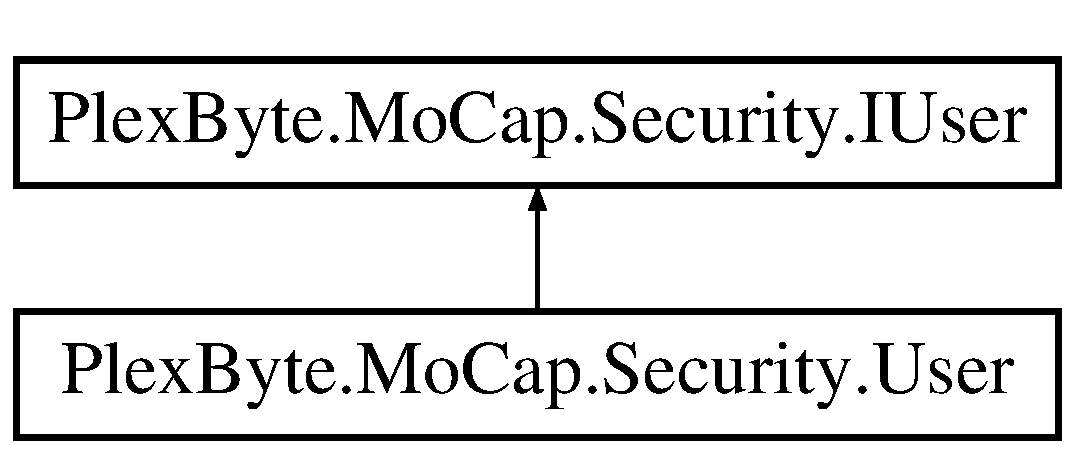
\includegraphics[height=2.000000cm]{interface_plex_byte_1_1_mo_cap_1_1_security_1_1_i_user}
\end{center}
\end{figure}
\subsection*{Properties}
\begin{DoxyCompactItemize}
\item 
string \hyperlink{interface_plex_byte_1_1_mo_cap_1_1_security_1_1_i_user_ab9deb17662dc2e4af4c794388fd1ef96}{Id}\hspace{0.3cm}{\ttfamily  \mbox{[}get\mbox{]}}
\item 
string \hyperlink{interface_plex_byte_1_1_mo_cap_1_1_security_1_1_i_user_a626a3fa1b5447931df4a99b12236d4d0}{Person\+Id}\hspace{0.3cm}{\ttfamily  \mbox{[}get\mbox{]}}
\item 
string \hyperlink{interface_plex_byte_1_1_mo_cap_1_1_security_1_1_i_user_a1e8c48f8a1f3fee58333fd586064e3fb}{Username}\hspace{0.3cm}{\ttfamily  \mbox{[}get, set\mbox{]}}
\item 
string \hyperlink{interface_plex_byte_1_1_mo_cap_1_1_security_1_1_i_user_aa2130f9b3edc6b7f08f40787486c841f}{Password}\hspace{0.3cm}{\ttfamily  \mbox{[}get, set\mbox{]}}
\end{DoxyCompactItemize}


\subsection{Detailed Description}


Definition at line 10 of file I\+User.\+cs.



\subsection{Property Documentation}
\index{Plex\+Byte\+::\+Mo\+Cap\+::\+Security\+::\+I\+User@{Plex\+Byte\+::\+Mo\+Cap\+::\+Security\+::\+I\+User}!Id@{Id}}
\index{Id@{Id}!Plex\+Byte\+::\+Mo\+Cap\+::\+Security\+::\+I\+User@{Plex\+Byte\+::\+Mo\+Cap\+::\+Security\+::\+I\+User}}
\subsubsection[{\texorpdfstring{Id}{Id}}]{\setlength{\rightskip}{0pt plus 5cm}string Plex\+Byte.\+Mo\+Cap.\+Security.\+I\+User.\+Id\hspace{0.3cm}{\ttfamily [get]}}\hypertarget{interface_plex_byte_1_1_mo_cap_1_1_security_1_1_i_user_ab9deb17662dc2e4af4c794388fd1ef96}{}\label{interface_plex_byte_1_1_mo_cap_1_1_security_1_1_i_user_ab9deb17662dc2e4af4c794388fd1ef96}


Definition at line 12 of file I\+User.\+cs.

\index{Plex\+Byte\+::\+Mo\+Cap\+::\+Security\+::\+I\+User@{Plex\+Byte\+::\+Mo\+Cap\+::\+Security\+::\+I\+User}!Password@{Password}}
\index{Password@{Password}!Plex\+Byte\+::\+Mo\+Cap\+::\+Security\+::\+I\+User@{Plex\+Byte\+::\+Mo\+Cap\+::\+Security\+::\+I\+User}}
\subsubsection[{\texorpdfstring{Password}{Password}}]{\setlength{\rightskip}{0pt plus 5cm}string Plex\+Byte.\+Mo\+Cap.\+Security.\+I\+User.\+Password\hspace{0.3cm}{\ttfamily [get]}, {\ttfamily [set]}}\hypertarget{interface_plex_byte_1_1_mo_cap_1_1_security_1_1_i_user_aa2130f9b3edc6b7f08f40787486c841f}{}\label{interface_plex_byte_1_1_mo_cap_1_1_security_1_1_i_user_aa2130f9b3edc6b7f08f40787486c841f}


Definition at line 15 of file I\+User.\+cs.

\index{Plex\+Byte\+::\+Mo\+Cap\+::\+Security\+::\+I\+User@{Plex\+Byte\+::\+Mo\+Cap\+::\+Security\+::\+I\+User}!Person\+Id@{Person\+Id}}
\index{Person\+Id@{Person\+Id}!Plex\+Byte\+::\+Mo\+Cap\+::\+Security\+::\+I\+User@{Plex\+Byte\+::\+Mo\+Cap\+::\+Security\+::\+I\+User}}
\subsubsection[{\texorpdfstring{Person\+Id}{PersonId}}]{\setlength{\rightskip}{0pt plus 5cm}string Plex\+Byte.\+Mo\+Cap.\+Security.\+I\+User.\+Person\+Id\hspace{0.3cm}{\ttfamily [get]}}\hypertarget{interface_plex_byte_1_1_mo_cap_1_1_security_1_1_i_user_a626a3fa1b5447931df4a99b12236d4d0}{}\label{interface_plex_byte_1_1_mo_cap_1_1_security_1_1_i_user_a626a3fa1b5447931df4a99b12236d4d0}


Definition at line 13 of file I\+User.\+cs.

\index{Plex\+Byte\+::\+Mo\+Cap\+::\+Security\+::\+I\+User@{Plex\+Byte\+::\+Mo\+Cap\+::\+Security\+::\+I\+User}!Username@{Username}}
\index{Username@{Username}!Plex\+Byte\+::\+Mo\+Cap\+::\+Security\+::\+I\+User@{Plex\+Byte\+::\+Mo\+Cap\+::\+Security\+::\+I\+User}}
\subsubsection[{\texorpdfstring{Username}{Username}}]{\setlength{\rightskip}{0pt plus 5cm}string Plex\+Byte.\+Mo\+Cap.\+Security.\+I\+User.\+Username\hspace{0.3cm}{\ttfamily [get]}, {\ttfamily [set]}}\hypertarget{interface_plex_byte_1_1_mo_cap_1_1_security_1_1_i_user_a1e8c48f8a1f3fee58333fd586064e3fb}{}\label{interface_plex_byte_1_1_mo_cap_1_1_security_1_1_i_user_a1e8c48f8a1f3fee58333fd586064e3fb}


Definition at line 14 of file I\+User.\+cs.



The documentation for this interface was generated from the following file\+:\begin{DoxyCompactItemize}
\item 
D\+:/\+Users/\+Christian\+B/\+Documents/\+\_\+\+H\+F Infomatik/\+Git\+Hub\+\_\+\+Repos/\+Mo\+Cap/\+Plex\+Byte.\+Mo\+Cap/\+Plex\+Byte.\+Mo\+Cap.\+Security/\hyperlink{_i_user_8cs}{I\+User.\+cs}\end{DoxyCompactItemize}

\hypertarget{class_plex_byte_1_1_mo_cap_1_1_security_1_1_user}{}\section{Plex\+Byte.\+Mo\+Cap.\+Security.\+User Class Reference}
\label{class_plex_byte_1_1_mo_cap_1_1_security_1_1_user}\index{Plex\+Byte.\+Mo\+Cap.\+Security.\+User@{Plex\+Byte.\+Mo\+Cap.\+Security.\+User}}
Inheritance diagram for Plex\+Byte.\+Mo\+Cap.\+Security.\+User\+:\begin{figure}[H]
\begin{center}
\leavevmode
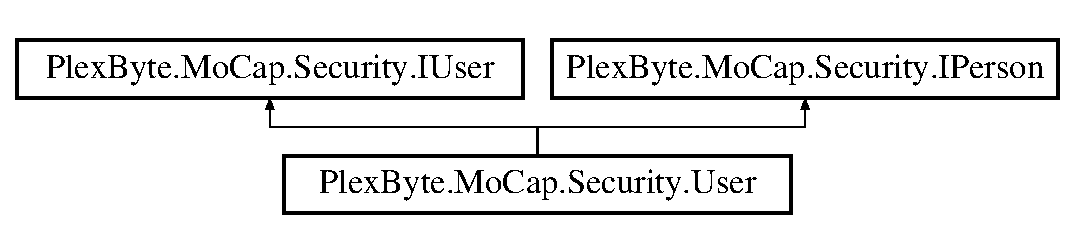
\includegraphics[height=2.000000cm]{class_plex_byte_1_1_mo_cap_1_1_security_1_1_user}
\end{center}
\end{figure}
\subsection*{Public Member Functions}
\begin{DoxyCompactItemize}
\item 
\hyperlink{class_plex_byte_1_1_mo_cap_1_1_security_1_1_user_a6d7f4d78f74f47c5f64e46ddf59043b1}{User} ()
\item 
\hyperlink{class_plex_byte_1_1_mo_cap_1_1_security_1_1_user_a3e87bb7b52983c083cd15886b61989a6}{User} (string p\+Id, string p\+Person\+Id, string p\+First\+Name, string p\+Last\+Name, string p\+Middle\+Name, string p\+Email\+Address, Date\+Time p\+Birth\+Date, Date\+Time p\+Created\+Date\+Time, Date\+Time p\+Modified\+Date\+Time, string p\+User\+Name, string p\+Password)
\end{DoxyCompactItemize}
\subsection*{Public Attributes}
\begin{DoxyCompactItemize}
\item 
string \hyperlink{class_plex_byte_1_1_mo_cap_1_1_security_1_1_user_a3e485cc6481d7d6c144e1f7c4818e611}{Id} =$>$ \+\_\+id
\item 
Date\+Time \hyperlink{class_plex_byte_1_1_mo_cap_1_1_security_1_1_user_a97a30ece2396be6bae1a88b47cf518d0}{Created\+Date\+Time} =$>$ \+\_\+created\+Date\+Time
\item 
string \hyperlink{class_plex_byte_1_1_mo_cap_1_1_security_1_1_user_a88a5440cb0d728dedb9f7fc59033f39e}{Person\+Id} =$>$ \+\_\+person\+Id
\end{DoxyCompactItemize}
\subsection*{Properties}
\begin{DoxyCompactItemize}
\item 
string \hyperlink{class_plex_byte_1_1_mo_cap_1_1_security_1_1_user_a96c459a22a26f039f17e2e84f486db36}{First\+Name}\hspace{0.3cm}{\ttfamily  \mbox{[}get, set\mbox{]}}
\item 
string \hyperlink{class_plex_byte_1_1_mo_cap_1_1_security_1_1_user_a9313e5d0899cddf88e7171da9fbb9e31}{Last\+Name}\hspace{0.3cm}{\ttfamily  \mbox{[}get, set\mbox{]}}
\item 
string \hyperlink{class_plex_byte_1_1_mo_cap_1_1_security_1_1_user_af6fccb21254c949d6f58f9011e2a25c4}{Middle\+Name}\hspace{0.3cm}{\ttfamily  \mbox{[}get, set\mbox{]}}
\item 
string \hyperlink{class_plex_byte_1_1_mo_cap_1_1_security_1_1_user_a0d766fcc163f7db495d4ef261a6ef02b}{Email\+Address}\hspace{0.3cm}{\ttfamily  \mbox{[}get, set\mbox{]}}
\item 
Date\+Time \hyperlink{class_plex_byte_1_1_mo_cap_1_1_security_1_1_user_a91c0564f89d8eb7eb0e19cf9bbf6f195}{Birthdate}\hspace{0.3cm}{\ttfamily  \mbox{[}get, set\mbox{]}}
\item 
Date\+Time \hyperlink{class_plex_byte_1_1_mo_cap_1_1_security_1_1_user_a412d3fe8c1013bd3ac76217717fe5814}{Modified\+Date\+Time}\hspace{0.3cm}{\ttfamily  \mbox{[}get, set\mbox{]}}
\item 
string \hyperlink{class_plex_byte_1_1_mo_cap_1_1_security_1_1_user_ab82f0c260e1863ade8f069da91405ab2}{Username}\hspace{0.3cm}{\ttfamily  \mbox{[}get, set\mbox{]}}
\item 
string \hyperlink{class_plex_byte_1_1_mo_cap_1_1_security_1_1_user_aa83a2d092f69dabaafb5c8d5646fa4f9}{Password}\hspace{0.3cm}{\ttfamily  \mbox{[}get, set\mbox{]}}
\end{DoxyCompactItemize}


\subsection{Detailed Description}


Definition at line 12 of file User.\+cs.



\subsection{Constructor \& Destructor Documentation}
\index{Plex\+Byte\+::\+Mo\+Cap\+::\+Security\+::\+User@{Plex\+Byte\+::\+Mo\+Cap\+::\+Security\+::\+User}!User@{User}}
\index{User@{User}!Plex\+Byte\+::\+Mo\+Cap\+::\+Security\+::\+User@{Plex\+Byte\+::\+Mo\+Cap\+::\+Security\+::\+User}}
\subsubsection[{\texorpdfstring{User()}{User()}}]{\setlength{\rightskip}{0pt plus 5cm}Plex\+Byte.\+Mo\+Cap.\+Security.\+User.\+User (
\begin{DoxyParamCaption}
{}
\end{DoxyParamCaption}
)}\hypertarget{class_plex_byte_1_1_mo_cap_1_1_security_1_1_user_a6d7f4d78f74f47c5f64e46ddf59043b1}{}\label{class_plex_byte_1_1_mo_cap_1_1_security_1_1_user_a6d7f4d78f74f47c5f64e46ddf59043b1}


Definition at line 32 of file User.\+cs.

\index{Plex\+Byte\+::\+Mo\+Cap\+::\+Security\+::\+User@{Plex\+Byte\+::\+Mo\+Cap\+::\+Security\+::\+User}!User@{User}}
\index{User@{User}!Plex\+Byte\+::\+Mo\+Cap\+::\+Security\+::\+User@{Plex\+Byte\+::\+Mo\+Cap\+::\+Security\+::\+User}}
\subsubsection[{\texorpdfstring{User(string p\+Id, string p\+Person\+Id, string p\+First\+Name, string p\+Last\+Name, string p\+Middle\+Name, string p\+Email\+Address, Date\+Time p\+Birth\+Date, Date\+Time p\+Created\+Date\+Time, Date\+Time p\+Modified\+Date\+Time, string p\+User\+Name, string p\+Password)}{User(string pId, string pPersonId, string pFirstName, string pLastName, string pMiddleName, string pEmailAddress, DateTime pBirthDate, DateTime pCreatedDateTime, DateTime pModifiedDateTime, string pUserName, string pPassword)}}]{\setlength{\rightskip}{0pt plus 5cm}Plex\+Byte.\+Mo\+Cap.\+Security.\+User.\+User (
\begin{DoxyParamCaption}
\item[{string}]{p\+Id, }
\item[{string}]{p\+Person\+Id, }
\item[{string}]{p\+First\+Name, }
\item[{string}]{p\+Last\+Name, }
\item[{string}]{p\+Middle\+Name, }
\item[{string}]{p\+Email\+Address, }
\item[{Date\+Time}]{p\+Birth\+Date, }
\item[{Date\+Time}]{p\+Created\+Date\+Time, }
\item[{Date\+Time}]{p\+Modified\+Date\+Time, }
\item[{string}]{p\+User\+Name, }
\item[{string}]{p\+Password}
\end{DoxyParamCaption}
)}\hypertarget{class_plex_byte_1_1_mo_cap_1_1_security_1_1_user_a3e87bb7b52983c083cd15886b61989a6}{}\label{class_plex_byte_1_1_mo_cap_1_1_security_1_1_user_a3e87bb7b52983c083cd15886b61989a6}


Definition at line 34 of file User.\+cs.



\subsection{Member Data Documentation}
\index{Plex\+Byte\+::\+Mo\+Cap\+::\+Security\+::\+User@{Plex\+Byte\+::\+Mo\+Cap\+::\+Security\+::\+User}!Created\+Date\+Time@{Created\+Date\+Time}}
\index{Created\+Date\+Time@{Created\+Date\+Time}!Plex\+Byte\+::\+Mo\+Cap\+::\+Security\+::\+User@{Plex\+Byte\+::\+Mo\+Cap\+::\+Security\+::\+User}}
\subsubsection[{\texorpdfstring{Created\+Date\+Time}{CreatedDateTime}}]{\setlength{\rightskip}{0pt plus 5cm}Date\+Time Plex\+Byte.\+Mo\+Cap.\+Security.\+User.\+Created\+Date\+Time =$>$ \+\_\+created\+Date\+Time}\hypertarget{class_plex_byte_1_1_mo_cap_1_1_security_1_1_user_a97a30ece2396be6bae1a88b47cf518d0}{}\label{class_plex_byte_1_1_mo_cap_1_1_security_1_1_user_a97a30ece2396be6bae1a88b47cf518d0}


Definition at line 22 of file User.\+cs.

\index{Plex\+Byte\+::\+Mo\+Cap\+::\+Security\+::\+User@{Plex\+Byte\+::\+Mo\+Cap\+::\+Security\+::\+User}!Id@{Id}}
\index{Id@{Id}!Plex\+Byte\+::\+Mo\+Cap\+::\+Security\+::\+User@{Plex\+Byte\+::\+Mo\+Cap\+::\+Security\+::\+User}}
\subsubsection[{\texorpdfstring{Id}{Id}}]{\setlength{\rightskip}{0pt plus 5cm}string Plex\+Byte.\+Mo\+Cap.\+Security.\+User.\+Id =$>$ \+\_\+id}\hypertarget{class_plex_byte_1_1_mo_cap_1_1_security_1_1_user_a3e485cc6481d7d6c144e1f7c4818e611}{}\label{class_plex_byte_1_1_mo_cap_1_1_security_1_1_user_a3e485cc6481d7d6c144e1f7c4818e611}


Definition at line 15 of file User.\+cs.

\index{Plex\+Byte\+::\+Mo\+Cap\+::\+Security\+::\+User@{Plex\+Byte\+::\+Mo\+Cap\+::\+Security\+::\+User}!Person\+Id@{Person\+Id}}
\index{Person\+Id@{Person\+Id}!Plex\+Byte\+::\+Mo\+Cap\+::\+Security\+::\+User@{Plex\+Byte\+::\+Mo\+Cap\+::\+Security\+::\+User}}
\subsubsection[{\texorpdfstring{Person\+Id}{PersonId}}]{\setlength{\rightskip}{0pt plus 5cm}string Plex\+Byte.\+Mo\+Cap.\+Security.\+User.\+Person\+Id =$>$ \+\_\+person\+Id}\hypertarget{class_plex_byte_1_1_mo_cap_1_1_security_1_1_user_a88a5440cb0d728dedb9f7fc59033f39e}{}\label{class_plex_byte_1_1_mo_cap_1_1_security_1_1_user_a88a5440cb0d728dedb9f7fc59033f39e}


Definition at line 24 of file User.\+cs.



\subsection{Property Documentation}
\index{Plex\+Byte\+::\+Mo\+Cap\+::\+Security\+::\+User@{Plex\+Byte\+::\+Mo\+Cap\+::\+Security\+::\+User}!Birthdate@{Birthdate}}
\index{Birthdate@{Birthdate}!Plex\+Byte\+::\+Mo\+Cap\+::\+Security\+::\+User@{Plex\+Byte\+::\+Mo\+Cap\+::\+Security\+::\+User}}
\subsubsection[{\texorpdfstring{Birthdate}{Birthdate}}]{\setlength{\rightskip}{0pt plus 5cm}Date\+Time Plex\+Byte.\+Mo\+Cap.\+Security.\+User.\+Birthdate\hspace{0.3cm}{\ttfamily [get]}, {\ttfamily [set]}}\hypertarget{class_plex_byte_1_1_mo_cap_1_1_security_1_1_user_a91c0564f89d8eb7eb0e19cf9bbf6f195}{}\label{class_plex_byte_1_1_mo_cap_1_1_security_1_1_user_a91c0564f89d8eb7eb0e19cf9bbf6f195}


Definition at line 21 of file User.\+cs.

\index{Plex\+Byte\+::\+Mo\+Cap\+::\+Security\+::\+User@{Plex\+Byte\+::\+Mo\+Cap\+::\+Security\+::\+User}!Email\+Address@{Email\+Address}}
\index{Email\+Address@{Email\+Address}!Plex\+Byte\+::\+Mo\+Cap\+::\+Security\+::\+User@{Plex\+Byte\+::\+Mo\+Cap\+::\+Security\+::\+User}}
\subsubsection[{\texorpdfstring{Email\+Address}{EmailAddress}}]{\setlength{\rightskip}{0pt plus 5cm}string Plex\+Byte.\+Mo\+Cap.\+Security.\+User.\+Email\+Address\hspace{0.3cm}{\ttfamily [get]}, {\ttfamily [set]}}\hypertarget{class_plex_byte_1_1_mo_cap_1_1_security_1_1_user_a0d766fcc163f7db495d4ef261a6ef02b}{}\label{class_plex_byte_1_1_mo_cap_1_1_security_1_1_user_a0d766fcc163f7db495d4ef261a6ef02b}


Definition at line 20 of file User.\+cs.

\index{Plex\+Byte\+::\+Mo\+Cap\+::\+Security\+::\+User@{Plex\+Byte\+::\+Mo\+Cap\+::\+Security\+::\+User}!First\+Name@{First\+Name}}
\index{First\+Name@{First\+Name}!Plex\+Byte\+::\+Mo\+Cap\+::\+Security\+::\+User@{Plex\+Byte\+::\+Mo\+Cap\+::\+Security\+::\+User}}
\subsubsection[{\texorpdfstring{First\+Name}{FirstName}}]{\setlength{\rightskip}{0pt plus 5cm}string Plex\+Byte.\+Mo\+Cap.\+Security.\+User.\+First\+Name\hspace{0.3cm}{\ttfamily [get]}, {\ttfamily [set]}}\hypertarget{class_plex_byte_1_1_mo_cap_1_1_security_1_1_user_a96c459a22a26f039f17e2e84f486db36}{}\label{class_plex_byte_1_1_mo_cap_1_1_security_1_1_user_a96c459a22a26f039f17e2e84f486db36}


Definition at line 17 of file User.\+cs.

\index{Plex\+Byte\+::\+Mo\+Cap\+::\+Security\+::\+User@{Plex\+Byte\+::\+Mo\+Cap\+::\+Security\+::\+User}!Last\+Name@{Last\+Name}}
\index{Last\+Name@{Last\+Name}!Plex\+Byte\+::\+Mo\+Cap\+::\+Security\+::\+User@{Plex\+Byte\+::\+Mo\+Cap\+::\+Security\+::\+User}}
\subsubsection[{\texorpdfstring{Last\+Name}{LastName}}]{\setlength{\rightskip}{0pt plus 5cm}string Plex\+Byte.\+Mo\+Cap.\+Security.\+User.\+Last\+Name\hspace{0.3cm}{\ttfamily [get]}, {\ttfamily [set]}}\hypertarget{class_plex_byte_1_1_mo_cap_1_1_security_1_1_user_a9313e5d0899cddf88e7171da9fbb9e31}{}\label{class_plex_byte_1_1_mo_cap_1_1_security_1_1_user_a9313e5d0899cddf88e7171da9fbb9e31}


Definition at line 18 of file User.\+cs.

\index{Plex\+Byte\+::\+Mo\+Cap\+::\+Security\+::\+User@{Plex\+Byte\+::\+Mo\+Cap\+::\+Security\+::\+User}!Middle\+Name@{Middle\+Name}}
\index{Middle\+Name@{Middle\+Name}!Plex\+Byte\+::\+Mo\+Cap\+::\+Security\+::\+User@{Plex\+Byte\+::\+Mo\+Cap\+::\+Security\+::\+User}}
\subsubsection[{\texorpdfstring{Middle\+Name}{MiddleName}}]{\setlength{\rightskip}{0pt plus 5cm}string Plex\+Byte.\+Mo\+Cap.\+Security.\+User.\+Middle\+Name\hspace{0.3cm}{\ttfamily [get]}, {\ttfamily [set]}}\hypertarget{class_plex_byte_1_1_mo_cap_1_1_security_1_1_user_af6fccb21254c949d6f58f9011e2a25c4}{}\label{class_plex_byte_1_1_mo_cap_1_1_security_1_1_user_af6fccb21254c949d6f58f9011e2a25c4}


Definition at line 19 of file User.\+cs.

\index{Plex\+Byte\+::\+Mo\+Cap\+::\+Security\+::\+User@{Plex\+Byte\+::\+Mo\+Cap\+::\+Security\+::\+User}!Modified\+Date\+Time@{Modified\+Date\+Time}}
\index{Modified\+Date\+Time@{Modified\+Date\+Time}!Plex\+Byte\+::\+Mo\+Cap\+::\+Security\+::\+User@{Plex\+Byte\+::\+Mo\+Cap\+::\+Security\+::\+User}}
\subsubsection[{\texorpdfstring{Modified\+Date\+Time}{ModifiedDateTime}}]{\setlength{\rightskip}{0pt plus 5cm}Date\+Time Plex\+Byte.\+Mo\+Cap.\+Security.\+User.\+Modified\+Date\+Time\hspace{0.3cm}{\ttfamily [get]}, {\ttfamily [set]}}\hypertarget{class_plex_byte_1_1_mo_cap_1_1_security_1_1_user_a412d3fe8c1013bd3ac76217717fe5814}{}\label{class_plex_byte_1_1_mo_cap_1_1_security_1_1_user_a412d3fe8c1013bd3ac76217717fe5814}


Definition at line 23 of file User.\+cs.

\index{Plex\+Byte\+::\+Mo\+Cap\+::\+Security\+::\+User@{Plex\+Byte\+::\+Mo\+Cap\+::\+Security\+::\+User}!Password@{Password}}
\index{Password@{Password}!Plex\+Byte\+::\+Mo\+Cap\+::\+Security\+::\+User@{Plex\+Byte\+::\+Mo\+Cap\+::\+Security\+::\+User}}
\subsubsection[{\texorpdfstring{Password}{Password}}]{\setlength{\rightskip}{0pt plus 5cm}string Plex\+Byte.\+Mo\+Cap.\+Security.\+User.\+Password\hspace{0.3cm}{\ttfamily [get]}, {\ttfamily [set]}}\hypertarget{class_plex_byte_1_1_mo_cap_1_1_security_1_1_user_aa83a2d092f69dabaafb5c8d5646fa4f9}{}\label{class_plex_byte_1_1_mo_cap_1_1_security_1_1_user_aa83a2d092f69dabaafb5c8d5646fa4f9}


Definition at line 26 of file User.\+cs.

\index{Plex\+Byte\+::\+Mo\+Cap\+::\+Security\+::\+User@{Plex\+Byte\+::\+Mo\+Cap\+::\+Security\+::\+User}!Username@{Username}}
\index{Username@{Username}!Plex\+Byte\+::\+Mo\+Cap\+::\+Security\+::\+User@{Plex\+Byte\+::\+Mo\+Cap\+::\+Security\+::\+User}}
\subsubsection[{\texorpdfstring{Username}{Username}}]{\setlength{\rightskip}{0pt plus 5cm}string Plex\+Byte.\+Mo\+Cap.\+Security.\+User.\+Username\hspace{0.3cm}{\ttfamily [get]}, {\ttfamily [set]}}\hypertarget{class_plex_byte_1_1_mo_cap_1_1_security_1_1_user_ab82f0c260e1863ade8f069da91405ab2}{}\label{class_plex_byte_1_1_mo_cap_1_1_security_1_1_user_ab82f0c260e1863ade8f069da91405ab2}


Definition at line 25 of file User.\+cs.



The documentation for this class was generated from the following file\+:\begin{DoxyCompactItemize}
\item 
D\+:/\+Users/\+Christian\+B/\+Documents/\+\_\+\+H\+F Infomatik/\+Git\+Hub\+\_\+\+Repos/\+Mo\+Cap/\+Plex\+Byte.\+Mo\+Cap/\+Plex\+Byte.\+Mo\+Cap.\+Security/\hyperlink{_user_8cs}{User.\+cs}\end{DoxyCompactItemize}

\chapter{File Documentation}
\hypertarget{_i_person_8cs}{}\section{D\+:/\+Users/\+Christian\+B/\+Documents/\+\_\+\+HF Infomatik/\+Git\+Hub\+\_\+\+Repos/\+Mo\+Cap/\+Plex\+Byte.Mo\+Cap/\+Plex\+Byte.Mo\+Cap.\+Security/\+I\+Person.cs File Reference}
\label{_i_person_8cs}\index{D\+:/\+Users/\+Christian\+B/\+Documents/\+\_\+\+H\+F Infomatik/\+Git\+Hub\+\_\+\+Repos/\+Mo\+Cap/\+Plex\+Byte.\+Mo\+Cap/\+Plex\+Byte.\+Mo\+Cap.\+Security/\+I\+Person.\+cs@{D\+:/\+Users/\+Christian\+B/\+Documents/\+\_\+\+H\+F Infomatik/\+Git\+Hub\+\_\+\+Repos/\+Mo\+Cap/\+Plex\+Byte.\+Mo\+Cap/\+Plex\+Byte.\+Mo\+Cap.\+Security/\+I\+Person.\+cs}}
\subsection*{Classes}
\begin{DoxyCompactItemize}
\item 
interface \hyperlink{interface_plex_byte_1_1_mo_cap_1_1_security_1_1_i_person}{Plex\+Byte.\+Mo\+Cap.\+Security.\+I\+Person}
\end{DoxyCompactItemize}
\subsection*{Namespaces}
\begin{DoxyCompactItemize}
\item 
namespace \hyperlink{namespace_plex_byte_1_1_mo_cap_1_1_security}{Plex\+Byte.\+Mo\+Cap.\+Security}
\end{DoxyCompactItemize}

\hypertarget{_i_user_8cs}{}\section{D\+:/\+Users/\+Christian\+B/\+Documents/\+\_\+\+HF Infomatik/\+Git\+Hub\+\_\+\+Repos/\+Mo\+Cap/\+Plex\+Byte.Mo\+Cap/\+Plex\+Byte.Mo\+Cap.\+Security/\+I\+User.cs File Reference}
\label{_i_user_8cs}\index{D\+:/\+Users/\+Christian\+B/\+Documents/\+\_\+\+H\+F Infomatik/\+Git\+Hub\+\_\+\+Repos/\+Mo\+Cap/\+Plex\+Byte.\+Mo\+Cap/\+Plex\+Byte.\+Mo\+Cap.\+Security/\+I\+User.\+cs@{D\+:/\+Users/\+Christian\+B/\+Documents/\+\_\+\+H\+F Infomatik/\+Git\+Hub\+\_\+\+Repos/\+Mo\+Cap/\+Plex\+Byte.\+Mo\+Cap/\+Plex\+Byte.\+Mo\+Cap.\+Security/\+I\+User.\+cs}}
\subsection*{Classes}
\begin{DoxyCompactItemize}
\item 
interface \hyperlink{interface_plex_byte_1_1_mo_cap_1_1_security_1_1_i_user}{Plex\+Byte.\+Mo\+Cap.\+Security.\+I\+User}
\end{DoxyCompactItemize}
\subsection*{Namespaces}
\begin{DoxyCompactItemize}
\item 
namespace \hyperlink{namespace_plex_byte_1_1_mo_cap_1_1_security}{Plex\+Byte.\+Mo\+Cap.\+Security}
\end{DoxyCompactItemize}

\hypertarget{_user_8cs}{}\section{D\+:/\+Users/\+Christian\+B/\+Documents/\+\_\+\+HF Infomatik/\+Git\+Hub\+\_\+\+Repos/\+Mo\+Cap/\+Plex\+Byte.Mo\+Cap/\+Plex\+Byte.Mo\+Cap.\+Security/\+User.cs File Reference}
\label{_user_8cs}\index{D\+:/\+Users/\+Christian\+B/\+Documents/\+\_\+\+H\+F Infomatik/\+Git\+Hub\+\_\+\+Repos/\+Mo\+Cap/\+Plex\+Byte.\+Mo\+Cap/\+Plex\+Byte.\+Mo\+Cap.\+Security/\+User.\+cs@{D\+:/\+Users/\+Christian\+B/\+Documents/\+\_\+\+H\+F Infomatik/\+Git\+Hub\+\_\+\+Repos/\+Mo\+Cap/\+Plex\+Byte.\+Mo\+Cap/\+Plex\+Byte.\+Mo\+Cap.\+Security/\+User.\+cs}}
\subsection*{Classes}
\begin{DoxyCompactItemize}
\item 
class \hyperlink{class_plex_byte_1_1_mo_cap_1_1_security_1_1_user}{Plex\+Byte.\+Mo\+Cap.\+Security.\+User}
\end{DoxyCompactItemize}
\subsection*{Namespaces}
\begin{DoxyCompactItemize}
\item 
namespace \hyperlink{namespace_plex_byte_1_1_mo_cap_1_1_security}{Plex\+Byte.\+Mo\+Cap.\+Security}
\end{DoxyCompactItemize}

%--- End generated contents ---

% Index
\backmatter
\newpage
\phantomsection
\clearemptydoublepage
\addcontentsline{toc}{chapter}{Index}
\printindex

\end{document}
